\documentclass[tikz, border=3pt]{standalone}

\usepackage{tikz}
\usetikzlibrary{calc}

\begin{document}
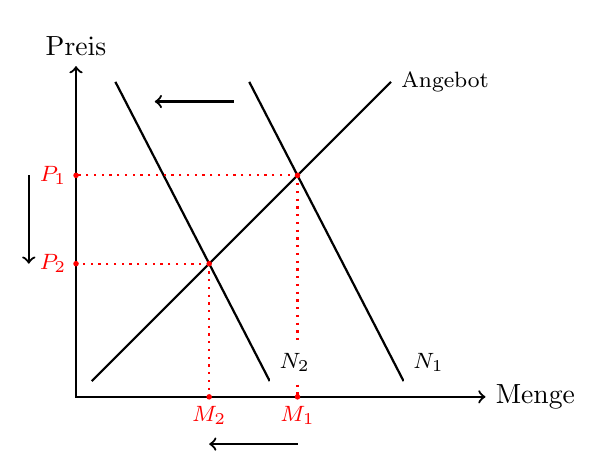
\begin{tikzpicture}
	
	\draw[thick] (.2,.2) coordinate (a1) -- (4,4) coordinate (a2) node[right, text width=5em] {\footnotesize Angebot};
	
	\draw[thick] (.5,4) coordinate (b1) -- (2.46, .2) coordinate (b2);
	\draw[thick] (2.2,4) coordinate (c1) -- (4.16, .2) coordinate (c2);
	
	\fill[red] (intersection cs: first line={(a1) -- (a2)}, second line={(c1) -- (c2)}) coordinate (i1) circle (1pt);
	\fill[red] (intersection cs: first line={(a1) -- (a2)}, second line={(b1) -- (b2)}) coordinate (i2) circle (1pt);
	
	
	
	\draw[thick, red, dotted] let \p1 = (i1) in (i1) -- (\x1,0) coordinate (e1);
	\draw[thick, red, dotted] let \p1 = (i1) in (i1) -- (0,\y1) coordinate (e3);
	
	\draw[thick, red, dotted] let \p1 = (i2) in (i2) -- (\x1,0) coordinate (e2);
	\draw[thick, red, dotted] let \p1 = (i2) in (i2) -- (0,\y1) coordinate (e4);
	

	\draw [<->, thick] (0,4.2) node (yaxis) [above] {Preis} |- (5.2,0) node (xaxis) [right] {Menge};
	
	\draw[] (b2) node[above right, fill=white] {\footnotesize $N_2$};
	\draw[] (c2) node[above right, fill=white] {\footnotesize $N_1$};
	
	\draw[->, thick] let \p1 = (e3), \p2 = (e4) in (-.6, \y1) -- (-.6, \y2);
	\draw[->, thick] let \p1 = (e1), \p2 = (e2) in (\x1,-.6) -- (\x2, -.6);
	
	\draw[->, thick] (2,3.75) -- (1,3.75);
	
	
	\fill[red] (e1) circle (1pt)  node[below] {\footnotesize $M_1$};
	\fill[red] (e2) circle (1pt)  node[below] {\footnotesize $M_2$};
	
	\fill[red] (e3) circle (1pt)  node[left] {\footnotesize $P_1$};
	\fill[red] (e4) circle (1pt)  node[left] {\footnotesize $P_2$};
	
\end{tikzpicture}
\end{document} 